\documentclass[final]{anthology-ch}

\usepackage{booktabs}
\usepackage{graphicx}

\usepackage{cleveref}
\usepackage{enumitem}

\title{Classifying Name-Date and Year Figures in Mixtec Codices}

\author{Girish Salunke} [
orcid=0009-0005-3472-7720
]

\author[1]{Christopher Driggers-Ellis}[
orcid=0009-0006-8063-7571
]

\author[1]{Christan Grant}[
orcid=0000-0002-6684-3620
]

\affiliation{1}{Computer \& Information Science \& Engineering, University of Florida, Gainesville, FL, USA}

\keywords{Mixtec Codices,
Vision Transformers,
Semasiography,
Cultural Heritage,
Image Classification,
Binary Classification,
Mesoamerican Studies, Mesoamerican Manuscripts,
Pictographic Manuscripts,
Semasiographic
Manuscripts,
Pictographic Writing}

\pubyear{2025}
\pubvolume{3}
\pagestart{1210}
\pageend{1218}
\conferencename{Computational Humanities Research 2025}
\conferenceeditors{Taylor Arnold, Margherita Fantoli, and Ruben Ros}
\doi{10.63744/eNge3Gj1LSHb}
\paperorder{71}

\addbibresource{bibliography.bib}

\begin{document}

\maketitle

\begin{abstract}
The Mixtec codices are precolonial and early colonial Mesoamerican manuscripts that use a semasiographic writing system to record historical, genealogical, and cosmological information. Decoding these manuscripts is uniquely challenging due to their non-linear structure and symbolic complexity. In this work, we introduce a novel application of Vision Transformers (ViTs) to classify key elements of Mixtec writing. Our classification pipeline involves a type classifier to distinguish between year and name-date symbols, followed by a symbol classifier to identify calendrical signs, and finally, a numerical bead counter. This pipeline tackles the challenge of high intra-class variability in hand-drawn symbols and separates the complex, often overlapping symbolic glyphs from their numerical components. Our results show a surprising dichotomy: ViTs achieve an F1 score greater than 0.9 in symbol classification but struggle with the counting task, where the F1 score is about 0.22. This contrast highlights a core architectural trade-off in Vision Transformers: their global attention mechanism helps with holistic pattern recognition, but it hinders fine-grained spatial localization. This insight clarifies both the potential and limitations of using ViTs to decode semasiographic texts, which can help guide more targeted applications in cultural heritage preservation. Our code is available here: \url{https://github.com/ufdatastudio/mixtec-namedate-classifiers}
\end{abstract}

\section{Introduction}

The Mixtec codices are manuscripts produced by the Mixtec civilization of pre-colonial and early colonial Mesoamerica.
These codices use a semasiographic writing system—conveying meaning through images rather than phonetic or logographic symbols.
Rich with imagery representing historical events, deities, rulers, and calendrical information, the codices function as complex narrative documents that communicate cultural knowledge independently of phonetic representation.
Analyzing these narratives is fundamental to preserving the cultural memory of the Mixtec people and provides a vital indigenous perspective on Mesoamerican history. Understanding these intricate systems is crucial not only for the Mixtec community but also for broader Mesoamerican studies, offering unique insights into pre-Columbian thought, history, and social structures that are often absent from colonial records.

Deciphering Mixtec writing is challenging due to its semasiographic nature, limited annotated data, and nonlinear reading order, often guided by visual cues within the codices.
Recent advances in computer vision have proven effective for historical document analysis; however, existing methods are largely designed for phonetic scripts.
The decoding of semasiographic systems remains an underexplored area, particularly in low-resource contexts where symbol sets are small but semantically dense~\cite{iglesia2021maya}.

In this work, we explore the use of Vision Transformers (ViTs)—a class of transformer-based models adapted for image understanding—to decode key elements of Mixtec codices.
Our goal is to classify name-dates and year symbols, which are central to interpreting the narratives in these manuscripts.
This paper outlines our contributions, including: (1) proposing a novel ViT-based pipeline for semasiographic symbol classification, (2) demonstrating the efficacy of ViTs for distinguishing complex glyphs in low-resource settings, and (3) highlighting the architectural limitations of ViTs for fine-grained counting tasks, which is critical for future research in computational cultural heritage.

\subsection{Background}
The Mixtec calendar system, adapted from the broader Mesoamerican tradition, is built on a 260-day Sacred Calendar (Tonalpohualli) and a 365-day Solar Calendar (Xiuhpohualli)~\cite{williams2013complete}. Individuals are named for days in the Sacred Calendar, with the associated date typically corresponding to their date of birth. These name-dates are composed of a number (1–13) and one of 20 calendrical day signs (e.g., ``8 Deer,'' ``4 Reed'')~\cite{boone2000stories,williams2013complete}.
These name-dates serve as proper names for historical figures, gods, or ancestors and often recur across multiple codices.
Similarly, years are marked using a combination of a number (1--13) and one of four year signs (Rabbit, Reed, House, Flint), forming a 52-year Calendar Round used for historical chronology \cite{boone2000stories,williams2013complete}.

Visually, name-dates and year symbols share structural similarities, typically consisting of a numeric prefix depicted as a series of small ``beads''—paired with a pictorial glyph. However, their \textit{semantic roles} differ: name-dates identify individuals (typically based on the calendar day of birth), while year symbols serve as chronological anchors for historical events. The presence of the \textit{year AO glyph} is used to disambiguate these cases in several codices, including the Zouche-Nuttall.\footnote{The ``AO'' year sign, also known as the \textit{annus obitus} or ``year-of'' glyph, is a conventional Mixtec symbol that marks a calendrical expression as a reference to a year rather than a personal name.
It often appears as a stylized circle or cartouche enclosing the year symbol \cite{boone2000stories,williams2013complete}.}
\Cref{fig:codex} visually illustrates this distinction, with name-dates highlighted using red squares and year symbols marked in green.
Importantly, the term \textit{name-date} also applies to instances where a specific calendar day (e.g., ``8 Deer'') is appended to a year (e.g., ``3 Flint'') to record the exact date of a historical event. In such cases, the name-date functions not as a personal identifier but as a temporal marker within the 52-year calendar round.
\begin{figure}[t!]
\centering
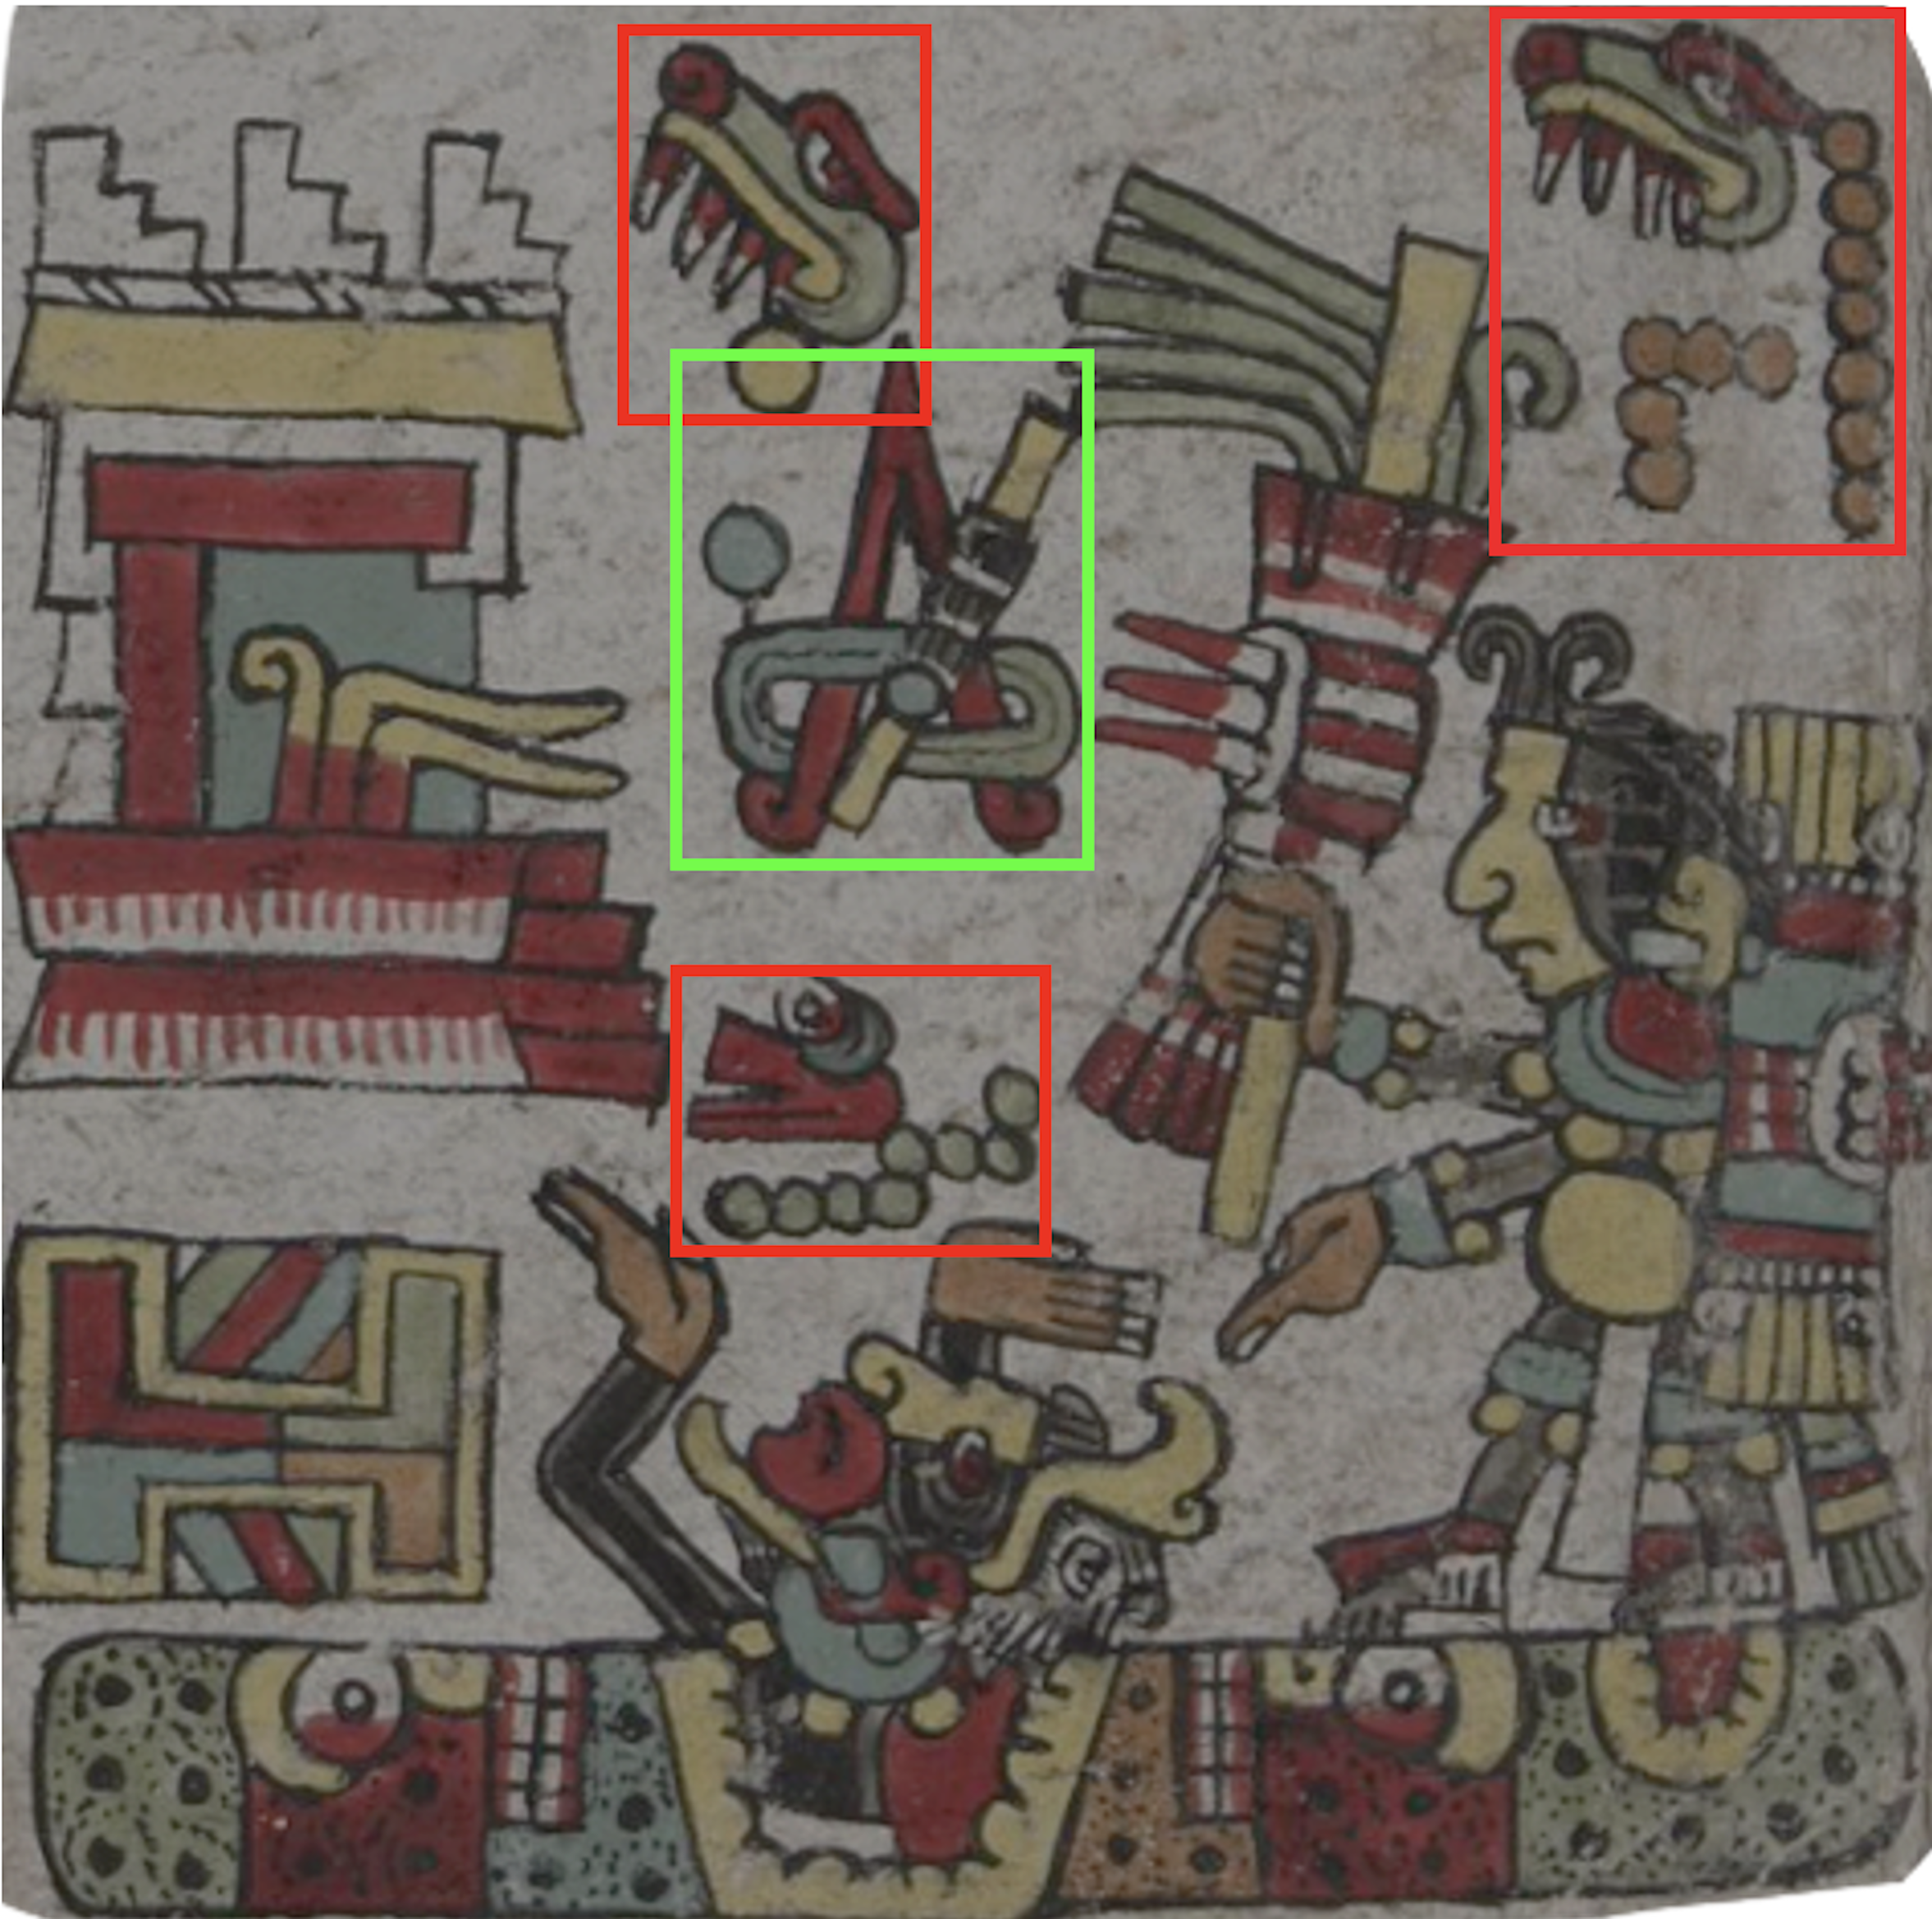
\includegraphics[width=0.35\linewidth]{figures/MixtecCodex.png}
\caption{Red squares highlight name-dates, which identify individuals through a combination of a day sign and number. The green square highlights a year symbol, which serves as a chronological marker within the narrative. Provided courtesy of the British Museum.}
\label{fig:codex}
\end{figure}
Both types of symbols draw from the same visual inventory of calendrical signs and follow a similar structural format. This shared design creates considerable visual ambiguity, especially when the presence of the AO glyph is faint, damaged, or omitted. As a result, distinguishing between name-dates and year symbols is not only essential for determining \textit{who is depicted} and \textit{when an event occurred}, but also a non-trivial classification challenge that requires careful symbolic analysis~\cite{boone2000stories,williams2013complete}.

\begin{figure}[t!]
\centering
\includegraphics[width=0.95\linewidth]{figures/name-date-vs-year.png}
\caption{
Visual comparison of a \textbf{name-date} and a \textbf{year symbol with AO marker}. Both include a numerical prefix (beads) and a glyph (e.g., Rabbit or Reed), but the year symbol includes the AO marker, distinguishing it as a chronological reference rather than a personal identifier. Cropped from original images provided courtesy of the British Museum.
}
\label{fig:name-vs-year}
\end{figure}

To address this challenge, we propose a image classification sequence using ViTs. Figure \ref{fig:images-to-classifiers} illustrates this  using an example:
\begin{itemize}[noitemsep,nolistsep]
\item The \textbf{name-date/year classifier} distinguishes between name-dates and year symbols;
\item The \textbf{symbol classifier} identifies the calendrical glyph;
\item The \textbf{bead counter} module extracts the numerical prefix.
\end{itemize}

Our approach leverages transfer learning and data augmentation to address the limited size of the annotated corpus.
This study contributes to the growing body of research at the intersection of machine learning and cultural heritage, demonstrating how transformer-based architectures can assist in interpreting symbolic, non-phonetic writing ~\cite{zora265462, muther2023querying, FIORUCCI2020102}.

\section{Related Work}
Machine-based interpretation of historical manuscripts has long been an interdisciplinary challenge, at the intersection of computer vision, anthropology, and linguistics. Although considerable progress has been made in the analysis of phonetic scripts using OCR and handwriting recognition ~\cite{ocrhindi2013}, semasiographic systems, such as those found in Mesoamerican codices, require different approaches due to their non-linear structure and reliance on symbolic imagery.

Studies on Mesoamerican writing systems show that these codices follow strict conventions to depict years, dates, names, and individuals \cite{jansen1988mesoamerican,boone2000stories}. The Mixtec codices, in particular, use calendrical and genealogical references through symbols rather than phonetic text, making visual classification crucial for decipherment. Foundational ethnographic and iconographic analyses laid the groundwork for understanding how meaning is encoded through symbolic combinations of numbers and day or year glyphs \cite{boone2000stories,smith1973picturewriting}.

Recent computational work has begun to operationalize these iconographic insights.
One related work introduces a dataset of segmented figures from three Mixtec codices, Zouche-Nuttall, Selden, and Vindobonensis, and apply deep learning models (VGG-16 and ViT-B/16) to two binary classification tasks: gender and pose \cite{webber-etal-2024-analyzing}. Their experiments demonstrate that fine-tuned Vision Transformers outperform CNNs, particularly at higher learning rates, and that attention map analyses reveal alignment between model predictions and expert heuristics (e.g., visual cues like loincloths or skirts). Our work validates the feasibility deep learning approaches to low-resource cultural heritage datasets.

Name-dates function as identifiers usually assigned at birth according to the 260-day ritual calendar, while year symbols locate events within a 52-year cycle. Name-dates are essential for understanding who is involved and when an event occurred in the codices, bridging the gap between image analysis and historical understanding.
Related work explores attributes such as pose and gender to help identify individual figures \cite{webber-etal-2024-analyzing}.
In contrast, our classifiers interpret the temporal and referential structures that form the manuscript's narrative backbone.

Beyond Mixtec codices, other work in historical document analysis has applied deep learning to ancient Egyptian hieroglyphs~\cite{egptHeiroDL} and Mayan glyphs~\cite{Can2018HowTT}. However, these efforts often rely on large labeled datasets or exploit textual regularities not present in Mixtec imagery. Our use of Vision Transformers demonstrates the potential of transformer-based architectures for low-resource, symbolic domains like semasiographic scripts.

Particularly, our approach leverages Vision Transformers (ViTs) to offer a promising view of global visual context—particularly in cases where symbols are semantically rich but structurally ambiguous.
We decode symbolic elements in Mixtec codices by classifying their relevant semantic components including glyph type, identity, and number using ViTs fine-tuned via transfer learning (\Cref{fig:images-to-classifiers}).

\section{Methodology}

The visual complexity and symbolic structure of Mixtec codices require a tailored computational approach that can distinguish between semantically distinct yet visually similar glyphs. We develop a modular classification pipeline that isolates and analyzes key calendrical components, specifically name-dates and year symbols, using fine-tuned Vision Transformer (ViT) models. This methodology section outlines the architecture of our system, training strategy, and data preprocessing steps, providing a foundation for automated calendrical interpretation in semasiographic scripts.

\subsection{Overview of Classification Pipeline}\label{AA}
The input to our system is a cropped image segment from annotated Mixtec codices. The classification pipeline consists of the following components:

\begin{itemize}[noitemsep,nolistsep]
\item \textbf{Name-Date/Year Classifier}: Distinguishes whether a given symbol represents a year or a name by detecting the AO symbol.
\item \textbf{Symbol Classifier}: Identifies the glyph symbol, such as ``Rabbit,'' ``Reed,'' or ``Flint.''
\item \textbf{Bead Counter}: Predicts the numerical component (1–13) typically represented as a sequence of small circular marks or ``beads'' accompanying the main symbol.
\end{itemize}

Our classification pipeline is designed to decode calendrical symbols found in the Mixtec codices by identifying their type, symbolic content, and associated number. The input to this system consists of cropped image segments containing annotated name-date and year symbols, taken from the dataset introduced in~\cite{webber-etal-2024-analyzing}. This data set includes high-resolution scans of three Mixtec codices: Codex Zouche-Nuttall, Codex Selden, and Codex Vindobonensis Mexicanus I, and was initially annotated for figure-level classification tasks such as gender and pose. We extend this work by labeling symbolic units corresponding to Mixtec calendrical representations.

\begin{figure}[t!]
\centering
\includegraphics[width=0.8\linewidth]{figures/classifier_pipeline_figure.png}
\caption{Proposed classification pipeline: Input images are fed into independent classifiers: a Name-Date/Year Classifier determines the symbol's type, a Symbol Classifier identifies the calendrical glyph (e.g., Reed or House), and a Bead Counter extracts the associated numerical value. The outputs are then combined to form the complete calendrical interpretation, such as ``Name-Date Year 12 Reed'' or ``Year 9 House.''}
\label{fig:images-to-classifiers}
\end{figure}

\Cref{fig:images-to-classifiers} illustrates the proposed classification pipeline. Images are processed by three classifiers: the Name-Date/Year Classifier, the Symbol Classifier, and the Bead Counter. The Name-Date/Year Classifier determines whether the symbol represents a name-date or a year. Both categories share a common structure: a pictographic glyph accompanied by one or more small circular marks or ``beads'' representing a numerical value of 1 to 13, but differ in their semantic roles. To classify an input as a year, the model must detect the presence of the AO symbol. The Symbol Classifier identifies the glyph itself. For year symbols, the classifier classifies the glyph as one of four canonical symbols: Rabbit, Reed, House, or Flint—associated with the 365-day solar calendar. For name-dates, the classifier selects from a set of 20 day signs used in the 260-day ritual calendar (e.g., Deer, Jaguar, Rain, Flower)~\cite{williams2013complete}.

The Bead Counter, which counts the number of beads depicted alongside the glyph. This number completes the calendrical representation by forming a pair with the glyph's sign (e.g., ``8 Deer'' or ``3 Flint'', see \Cref{fig:name-vs-year}).

We implement each component in the pipeline using a fine-tuned Vision Transformer (ViT-B/16) model~\cite{dosovitskiy2021an} trained on task-specific subsets of the annotated symbol dataset.

\subsection{Vision Transformer Architecture}
We fine-tune a Vision Transformer (ViT-B/16) model~\cite{dosovitskiy2021an} for each of the classification tasks described in our pipeline.

This architecture is particularly effective in capturing both local and global visual dependencies, making it suitable for distinguishing the subtle symbolic differences present in Mixtec codices.

We initialize our ViT-B/16 models with default weights from the \texttt{torchvision.models} module. For each classification task—type identification (name-date vs year), glyph classification, and bead counting, we replace the original classification head with a task-specific linear layer. The backbone of the pre-trained ViT is frozen to preserve general visual features, while we train the classification head on our Mixtec symbol dataset.

We adopt cross-entropy loss and the Adam optimizer with a learning rate of 0.001. To enhance reproducibility, we fix random seeds and use the automated image pre-processing pipeline associated with the pre-trained ViT weights, including resizing, normalization, and color adjustments.

We perform fine-tuning using a single A100 GPU, with a batch size of 32 and up to 16 parallel data-loading workers. We trained each classifier for 10 epochs, as visual inspection of the loss curves in \Cref{fig:training-loss} indicated plateaus in training and test loss.

Given the limited size of our dataset, we employ transfer learning to leverage the representational power of ViTs pre-trained on large-scale natural image corpora.

\begin{figure}
\centering
\includegraphics[width=1\linewidth]{figures/loss_curves.png}
\caption{Loss Curves for ViT Classifiers - (a) Namedate-year, (b) Symbol Classifier, and (c) Bead Counter. Each subplot illustrates the progression of both training and testing loss over 10 epochs.}
\label{fig:training-loss}
\end{figure}

\subsection{Data Augmentation}

To enhance model generalization and mitigate overfitting due to limited training data, we apply four data augmentation techniques to the Mixtec symbol images. The dataset is partitioned into training and test sets in a 70:30 ratio, yielding 48,742 training images and 20,889 test images. Data augmentation is applied iteratively, with each augmentation technique performed sequentially. After each augmentation step, the augmented images are added to the existing dataset, progressively increasing the total number of images.

\begin{description}[noitemsep,nolistsep]
\item [{Random Rotation:}] Images are rotated at varying angles to simulate the diverse orientations in which symbols may appear across different codices.
\item \textbf{Color Jittering:} Controlled adjustments to brightness, contrast, and hue are applied to account for visual inconsistencies such as faded ink, aged parchment, and scanning artifacts.
\item [{Random Masking:}] Portions of the symbols are randomly occluded to encourage the model to learn discriminative features from partial inputs and improve resilience to damage or incomplete glyphs.
\item [{Oversampling of Underrepresented Classes:}] Classes with fewer examples (especially rarer day or year symbols) are augmented more heavily to balance the class distribution within the dataset.

\end{description}

These augmentations, improving the robustness of the classifiers to visual noise, partial occlusions, and layout inconsistencies commonly found in historical manuscripts.

\section{Results}

\Cref{tab:accuracy-summary} shows the test results after 10 epochs of training.
The \textit{type classifier} and \textit{symbol classifier} achieve better performance than \textit{bead counter}. The binary \textit{type classifier} achieves an F1 score >.90, and \textit{symbol classifier} achieves F1 score of 0.74 despite the complexity of classifying 20 visually similar glyphs. In contrast, \textit{bead counter} shows a >.50 gap between training and test accuracy, suggesting that Vision Transformers are ineffective for counting repetitive visual elements.

Vision Transformers (ViTs), while effective at symbolic classification, performed poorly in  \textit{bead counter} tests, with an F1 score of 0.22. The beads in the Mixtec codices are small, repetitive, and closely spaced, conditions that challenge ViTs, which lack the local spatial biases that convolutional networks naturally possess~\cite{d2021convit}.

\begin{table}[ht]
\centering
\begin{tabular}{cccccc}
\toprule
\textbf{Classifier} & \textbf{Train Accuracy} & \textbf{Test Accuracy} & \textbf{Precision} & \textbf{Recall} & \textbf{F1} \\
\midrule
Type Classifier & 0.9892 & 0.9795 & 0.9697  & 0.9209 & 0.9436  \\
Symbol Classifier & 0.9773 & 0.8562 & 0.7491 & 0.7318 & 0.7367 \\
Bead Counter & 0.7748 & 0.2589 &  0.2372 & 0.2201 & 0.2283  \\
\bottomrule
\end{tabular}
\caption{Training accuracy and test accuracy, precision, recall and F1 score for each classifier after 10 epochs.}
\label{tab:accuracy-summary}
\end{table}

\section{Discussion}

Our experiments demonstrate that ViTs can be effectively fine-tuned to classify symbolic components in Mixtec codices. The strong performance of the type and symbol classifiers suggests that ViTs are capable of modeling nuanced visual distinctions between glyph categories, even under limited data conditions~\cite{dosovitskiy2021an,webber-etal-2024-analyzing}.

However, ViTs performed poorly on the bead counting task, with an F1 score around 0.22. This is likely due to their patch-based processing and global attention mechanism, which makes them less suitable for tasks requiring fine-grained spatial precision~\cite{naseer2021intriguing}. Beads in Mixtec codices are small, repetitive, and closely spaced conditions that challenge ViTs, which lack the local spatial biases that convolutional networks naturally possess~\cite{d2021convit}. These results suggest that object detection or localization-based models (e.g., Faster R-CNN, YOLO) may be more appropriate for counting tasks in this domain~\cite{ren2015faster,redmon2016you}.

\section{Future Work}

The classifiers developed in this work—focused on identifying name-dates, year symbols, and their numeric prefixes serve as foundational components for building a machine interpreter capable of analyzing Mixtec codices at scale. When integrated with other visual classifiers, these modules can support more comprehensive semantic parsing of codical scenes.

Our current results are promising for symbolic classification; future work must explore more suitable models for tasks requiring fine-grained spatial reasoning, such as bead counting.
Object detection or segmentation-based architectures (e.g., YOLO, Mask R-CNN) may offer greater accuracy for localizing and enumerating repeated visual units like beads. Incorporating such models would strengthen the pipeline’s ability to extract structured temporal data from codices.

Finally, although our work focuses on the Mixtec codices, the underlying architecture and methodology are extensible to other low-resource semasiographic writing systems, such as Zapotec, Aztec, or Maya codices, where meaning is conveyed visually rather than phonetically. Future research will aim to generalize these classifiers across such systems.

\section{Limitations}

Several of the challenges we encountered reflect broader limitations previously identified in the study of Mixtec codices~\cite{webber-etal-2024-analyzing}, particularly those related to dataset scope and classification methodology. While the Mixtec civilization produced a rich corpus of codices, conquest and the passage of time have left only a few high-quality manuscripts~\cite{boone2000stories}. Although digitized versions of these codices support computational analysis, the limited number and stylistic variation of surviving sources constrain dataset diversity and generalizability.

Fine-tuning of ViTs from pre-trained weights introduces additional constraints. These models are initialized with parameters derived from large-scale image datasets outside the domain of Mesoamerican visual culture. As a result, they may carry latent biases that are not explicitly visible in classification output but could influence downstream tasks. We have not yet investigated the nature or extent of these inherited biases.

Furthermore, our model does not incorporate context. Symbols are classified in isolation, despite the fact that their meaning in the codices is often compositional. This limitation is particularly relevant for name-dates, which may function either as personal identifiers or as temporal markers depending on their placement within a scene. Without considering spatial and relational context, such as proximity to figures or year glyphs, ViTs may misinterpret what role a name-date plays.

Finally, we have not integrated feedback loops with domain experts or stakeholders in the Mixtec community but we hope this work will spur these necessary collaborations.

\printbibliography

\end{document}